\chapter{Drawing on Canvas}\label{canvas}

\epigraphhead[30]{
\epigraph{\hspace*{-.1cm}\itshape``Drawing is deception.''}%
{---M.C. Escher, cited by Bruno Ernst in The Magic Mirror of M.C. Escher}
}\index{Escher, M.C.}\index{CSS}\index{transform (CSS)}\index{DOM!graphics}

Browsers give us several ways to display \index{graphics}graphics. The simplest way is to use styles to position and color regular DOM elements. This can get you quite far, as the game in the \hyperref[game]{previous chapter} showed. By adding partially transparent background \index{image}images to the nodes, we can make them look exactly the way we want. It is even possible to rotate or skew nodes with the \lstinline`transform` style.

But we'd be using the DOM for something that it wasn't originally designed for. Some tasks, such as drawing a \index{line}line between arbitrary points, are extremely awkward to do with regular HTML elements.\index{SVG}\index{img (HTML tag)}

There are two alternatives. The first is DOM-based but utilizes \emph{Scalable Vector Graphics} (SVG), rather than HTML. Think of SVG as a \index{document}document-markup dialect that focuses on \index{shape}shapes rather than text. You can embed an SVG document directly in an HTML document or include it with an \lstinline`<img>` tag.\index{clearing}\index{DOM!graphics}\index{interface!canvas}

The second alternative is called a \emph{\index{canvas}canvas}. A canvas is a single DOM element that encapsulates a \index{picture}picture. It provides a programming interface for drawing \index{shape}shapes onto the space taken up by the node. The main difference between a canvas and an SVG picture is that in SVG the original description of the shapes is preserved so that they can be moved or resized at any time. A canvas, on the other hand, converts the shapes to \index{pixel}pixels (colored dots on a raster) as soon as they are drawn and does not remember what these pixels represent. The only way to move a shape on a canvas is to clear the canvas (or the part of the canvas around the shape) and redraw it with the shape in a new position.

\section{SVG}

This book will not go into \index{SVG}SVG in detail, but I will briefly explain how it works. At the \hyperref[canvas.graphics_tradeoffs]{end of the chapter}, I'll come back to the trade-offs that you must consider when deciding which \index{drawing}drawing mechanism is appropriate for a given application.

This is an HTML document with a simple SVG \index{picture}picture in it:

\begin{lstlisting}
<p>Normal HTML here.</p>
<svg xmlns="http://www.w3.org/2000/svg">
  <circle r="50" cx="50" cy="50" fill="red"/>
  <rect x="120" y="5" width="90" height="90"
        stroke="blue" fill="none"/>
</svg>
\end{lstlisting}
\noindent\index{circle (SVG tag)}\index{rect (SVG tag)}\index{XML namespace}\index{XML}\index{xmlns attribute}

The \lstinline`xmlns` attribute changes an element (and its children) to a different \emph{XML namespace}. This namespace, identified by a \index{URL}URL, specifies the dialect that we are currently speaking. The \lstinline`<circle>` and \lstinline`<rect>` tags, which do not exist in HTML, do have a meaning in SVG—they draw shapes using the style and position specified by their attributes.

The document is displayed like this:

\vskip 1.5ex
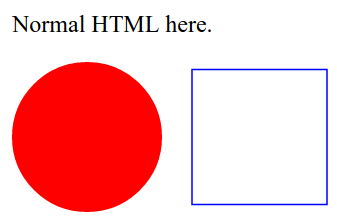
\includegraphics[width=4.5cm]{img/svg-demo.png}
\vskip 1.5ex\index{DOM!graphics}

These tags create DOM elements, just like HTML tags, that scripts can interact with. For example, this changes the \lstinline`<circle>` element to be \index{color}colored cyan instead:

\begin{lstlisting}
let circle = document.querySelector("circle");
circle.setAttribute("fill", "cyan");
\end{lstlisting}
\noindent

\section{The canvas element}\index{canvas!size}\index{canvas (HTML tag)}

Canvas \index{graphics}graphics can be drawn onto a \lstinline`<canvas>` element. You can give such an element \lstinline`width` and \lstinline`height` attributes to determine its size in \index{pixel}pixels.

A new canvas is empty, meaning it is entirely \index{transparent}transparent and thus shows up as empty space in the document.\index{2d (canvas context)}\index{webgl (canvas context)}\index{OpenGL}\index{canvas!context}\index{dimensions}\index{interface!canvas}

The \lstinline`<canvas>` tag is intended to allow different styles of \index{drawing}drawing. To get access to an actual drawing interface, we first need to create a \emph{\index{context}context}, an object whose methods provide the drawing interface. There are currently two widely supported drawing styles: \lstinline`"2d"` for two-dimensional graphics and \lstinline`"webgl"` for three-dimensional graphics through the OpenGL interface.\index{rendering}\index{graphics}\index{efficiency}

This book won't discuss WebGL—we'll stick to two dimensions. But if you are interested in three-dimensional graphics, I do encourage you to look into WebGL. It provides a direct interface to graphics hardware and allows you to render even complicated scenes efficiently, using JavaScript.\index{getContext method}\index{canvas!context}

You create a \index{context}context with the \lstinline`getContext` method on the \lstinline`<canvas>` DOM element.

\begin{lstlisting}
<p>Before canvas.</p>
<canvas width="120" height="60"></canvas>
<p>After canvas.</p>
<script>
  let canvas = document.querySelector("canvas");
  let context = canvas.getContext("2d");
  context.fillStyle = "red";
  context.fillRect(10, 10, 100, 50);
</script>
\end{lstlisting}
\noindent

After creating the context object, the example draws a red \index{rectangle}rectangle 100 \index{pixel}pixels wide and 50 pixels high, with its top-left corner at coordinates (10,10).

\vskip 1.5ex
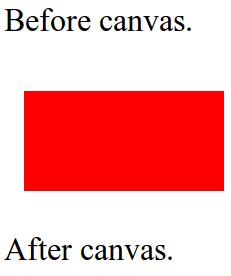
\includegraphics[width=2.5cm]{img/canvas_fill.png}
\vskip 1.5ex\index{SVG}\index{coordinates}

Just like in HTML (and SVG), the coordinate system that the canvas uses puts (0,0) at the top-left corner, and the positive y-\index{axis}axis goes down from there. So (10,10) is 10 pixels below and to the right of the top-left corner.

\label{canvas.fill_stroke}\section{Lines and surfaces}\index{filling}\index{stroking}\index{drawing}\index{SVG}

In the \index{canvas}canvas interface, a shape can be \emph{filled}, meaning its area is given a certain color or pattern, or it can be \emph{stroked}, which means a \index{line}line is drawn along its edge. The same terminology is used by SVG.\index{fillRect method}\index{strokeRect method}

The \lstinline`fillRect` method fills a \index{rectangle}rectangle. It takes first the x- and y-\index{coordinates}coordinates of the rectangle's top-left corner, then its width, and then its height. A similar method, \lstinline`strokeRect`, draws the \index{outline}outline of a rectangle.\index{state!of canvas}

Neither method takes any further parameters. The color of the fill, thickness of the stroke, and so on, are not determined by an argument to the method (as you might reasonably expect) but rather by properties of the context object.\index{filling}\index{fillStyle property}

The \lstinline`fillStyle` property controls the way shapes are filled. It can be set to a string that specifies a \index{color}color, using the color notation used by \index{CSS}CSS.\index{stroking}\index{line width}\index{strokeStyle property}\index{lineWidth property}\index{canvas}

The \lstinline`strokeStyle` property works similarly but determines the color used for a stroked line. The width of that line is determined by the \lstinline`lineWidth` property, which may contain any positive number.

\begin{lstlisting}
<canvas></canvas>
<script>
  let cx = document.querySelector("canvas").getContext("2d");
  cx.strokeStyle = "blue";
  cx.strokeRect(5, 5, 50, 50);
  cx.lineWidth = 5;
  cx.strokeRect(135, 5, 50, 50);
</script>
\end{lstlisting}
\noindent

This code draws two blue squares, using a thicker line for the second one.

\vskip 1.5ex
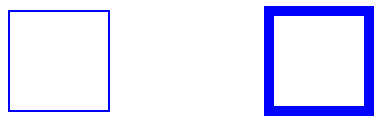
\includegraphics[width=5cm]{img/canvas_stroke.png}
\vskip 1.5ex\index{default value}\index{canvas!size}

When no \lstinline`width` or \lstinline`height` attribute is specified, as in the example, a canvas element gets a default width of 300 pixels and height of 150 pixels.

\section{Paths}\index{path!canvas}\index{interface!design}\index{canvas!path}

A path is a sequence of \index{line}lines. The 2D canvas interface takes a peculiar approach to describing such a path. It is done entirely through \index{side effect}side effects. Paths are not values that can be stored and passed around. Instead, if you want to do something with a path, you make a sequence of method calls to describe its shape.

\begin{lstlisting}
<canvas></canvas>
<script>
  let cx = document.querySelector("canvas").getContext("2d");
  cx.beginPath();
  for (let y = 10; y < 100; y += 10) {
    cx.moveTo(10, y);
    cx.lineTo(90, y);
  }
  cx.stroke();
</script>
\end{lstlisting}
\noindent\index{canvas}\index{stroke method}\index{lineTo method}\index{moveTo method}\index{shape}

This example creates a path with a number of horizontal \index{line}line segments and then strokes it using the \lstinline`stroke` method. Each segment created with \lstinline`lineTo` starts at the path's \emph{current} position. That position is usually the end of the last segment, unless \lstinline`moveTo` was called. In that case, the next segment would start at the position passed to \lstinline`moveTo`.

The path described by the previous program looks like this:

\vskip 1.5ex
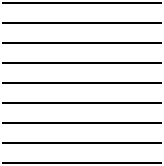
\includegraphics[width=2.1cm]{img/canvas_path.png}
\vskip 1.5ex\index{path!canvas}\index{filling}\index{path!closing}\index{fill method}

When filling a path (using the \lstinline`fill` method), each \index{shape}shape is filled separately. A path can contain multiple shapes—each \lstinline`moveTo` motion starts a new one. But the path needs to be \emph{closed} (meaning its start and end are in the same position) before it can be filled. If the path is not already closed, a line is added from its end to its start, and the shape enclosed by the completed path is filled.

\begin{lstlisting}
<canvas></canvas>
<script>
  let cx = document.querySelector("canvas").getContext("2d");
  cx.beginPath();
  cx.moveTo(50, 10);
  cx.lineTo(10, 70);
  cx.lineTo(90, 70);
  cx.fill();
</script>
\end{lstlisting}
\noindent

This example draws a filled triangle. Note that only two of the triangle's sides are explicitly drawn. The third, from the bottom-right corner back to the top, is implied and wouldn't be there when you stroke the path.

\vskip 1.5ex
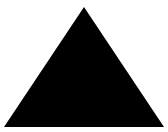
\includegraphics[width=2.2cm]{img/canvas_triangle.png}
\vskip 1.5ex\index{stroke method}\index{closePath method}\index{path!closing}\index{canvas}

You could also use the \lstinline`closePath` method to explicitly close a path by adding an actual \index{line}line segment back to the path's start. This segment \emph{is} drawn when stroking the path.

\section{Curves}\index{path!canvas}\index{canvas}\index{drawing}

A path may also contain \index{curve}curved \index{line}lines. These are unfortunately a bit more involved to draw.\index{quadraticCurveTo method}

The \lstinline`quadraticCurveTo` method draws a curve to a given point. To determine the curvature of the line, the method is given a \index{control
point}control
point as well as a destination point. Imagine this control point as \emph{attracting} the line, giving it its curve. The line won't go through the control point, but its direction at the start and end points will be such that a straight line in that direction would point toward the control point. The following example illustrates this:

\begin{lstlisting}
<canvas></canvas>
<script>
  let cx = document.querySelector("canvas").getContext("2d");
  cx.beginPath();
  cx.moveTo(10, 90);
  // control=(60,10) goal=(90,90)
  cx.quadraticCurveTo(60, 10, 90, 90);
  cx.lineTo(60, 10);
  cx.closePath();
  cx.stroke();
</script>
\end{lstlisting}
\noindent

It produces a path that looks like this:

\vskip 1.5ex
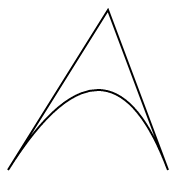
\includegraphics[width=2.3cm]{img/canvas_quadraticcurve.png}
\vskip 1.5ex\index{stroke method}

We draw a \index{quadratic curve}quadratic curve from the left to the right, with (60,10) as control point, and then draw two \index{line}line segments going through that control point and back to the start of the line. The result somewhat resembles a \emph{\index{Star Trek}Star Trek} insignia. You can see the effect of the control point: the lines leaving the lower corners start off in the direction of the control point and then \index{curve}curve toward their target.\index{canvas}\index{bezierCurveTo method}

The \lstinline`bezierCurveTo` method draws a similar kind of curve. Instead of a single \index{control point}control point, this one has two—one for each of the \index{line}line's endpoints. Here is a similar sketch to illustrate the behavior of such a curve:

\begin{lstlisting}
<canvas></canvas>
<script>
  let cx = document.querySelector("canvas").getContext("2d");
  cx.beginPath();
  cx.moveTo(10, 90);
  // control1=(10,10) control2=(90,10) goal=(50,90)
  cx.bezierCurveTo(10, 10, 90, 10, 50, 90);
  cx.lineTo(90, 10);
  cx.lineTo(10, 10);
  cx.closePath();
  cx.stroke();
</script>
\end{lstlisting}
\noindent

The two control points specify the direction at both ends of the curve. The farther they are away from their corresponding point, the more the curve will ``bulge'' in that direction.

\vskip 1.5ex
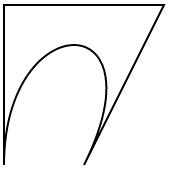
\includegraphics[width=2.2cm]{img/canvas_beziercurve.png}
\vskip 1.5ex\index{trial and error}

Such \index{curve}curves can be hard to work with—it's not always clear how to find the \index{control point}control points that provide the \index{shape}shape you are looking for. Sometimes you can compute them, and sometimes you'll just have to find a suitable value by trial and error.\index{arc method}\index{arc}

The \lstinline`arc` method is a way to draw a line that curves along the edge of a circle. It takes a pair of \index{coordinates}coordinates for the arc's center, a radius, and then a start angle and end angle.\index{pi}\index{Math.PI constant}

Those last two parameters make it possible to draw only part of the circle. The \index{angle}angles are measured in \index{radian}radians, not \index{degree}degrees. This means a full \index{circle}circle has an angle of 2π, or \lstinline`2 * Math.PI`, which is about 6.28. The angle starts counting at the point to the right of the circle's center and goes clockwise from there. You can use a start of 0 and an end bigger than 2π (say, 7) to draw a full circle.

\begin{lstlisting}
<canvas></canvas>
<script>
  let cx = document.querySelector("canvas").getContext("2d");
  cx.beginPath();
  // center=(50,50) radius=40 angle=0 to 7
  cx.arc(50, 50, 40, 0, 7);
  // center=(150,50) radius=40 angle=0 to ½π
  cx.arc(150, 50, 40, 0, 0.5 * Math.PI);
  cx.stroke();
</script>
\end{lstlisting}
\noindent\index{moveTo method}\index{arc method}\index{path! canvas}

The resulting picture contains a \index{line}line from the right of the full circle (first call to \lstinline`arc`) to the right of the quarter-\index{circle}circle (second call). Like other path-drawing methods, a line drawn with \lstinline`arc` is connected to the previous path segment. You can call \lstinline`moveTo` or start a new path to avoid this.

\vskip 1.5ex
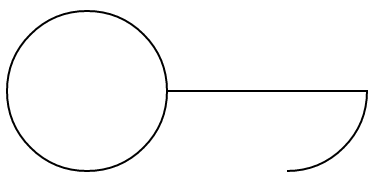
\includegraphics[width=4.9cm]{img/canvas_circle.png}
\vskip 1.5ex

\label{canvas.pie_chart}\section{Drawing a pie chart}\index{pie chart example}

Imagine you've just taken a \index{job}job at EconomiCorp, Inc., and your first assignment is to draw a pie chart of its customer satisfaction \index{survey}survey results.

The \lstinline`results` binding contains an array of objects that represent the survey responses.

\begin{lstlisting}
const results = [
  {name: "Satisfied", count: 1043, color: "lightblue"},
  {name: "Neutral", count: 563, color: "lightgreen"},
  {name: "Unsatisfied", count: 510, color: "pink"},
  {name: "No comment", count: 175, color: "silver"}
];
\end{lstlisting}
\noindent\index{pie chart example}

To draw a pie chart, we draw a number of pie slices, each made up of an \index{arc}arc and a pair of \index{line}lines to the center of that arc. We can compute the \index{angle}angle taken up by each arc by dividing a full circle (2π) by the total number of responses and then multiplying that number (the angle per response) by the number of people who picked a given choice.

\begin{lstlisting}
<canvas width="200" height="200"></canvas>
<script>
  let cx = document.querySelector("canvas").getContext("2d");
  let total = results
    .reduce((sum, {count}) => sum + count, 0);
  // Start at the top
  let currentAngle = -0.5 * Math.PI;
  for (let result of results) {
    let sliceAngle = (result.count / total) * 2 * Math.PI;
    cx.beginPath();
    // center=100,100, radius=100
    // from current angle, clockwise by slice's angle
    cx.arc(100, 100, 100,
           currentAngle, currentAngle + sliceAngle);
    currentAngle += sliceAngle;
    cx.lineTo(100, 100);
    cx.fillStyle = result.color;
    cx.fill();
  }
</script>
\end{lstlisting}
\noindent

This draws the following chart:

\vskip 1.5ex
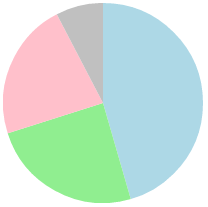
\includegraphics[width=5cm]{img/canvas_pie_chart.png}
\vskip 1.5ex

But a chart that doesn't tell us what the slices mean isn't very helpful. We need a way to draw text to the \index{canvas}canvas.

\section{Text}\index{stroking}\index{filling}\index{fillStyle property}\index{fillText method}\index{strokeText method}

A 2D canvas drawing context provides the methods \lstinline`fillText` and \lstinline`strokeText`. The latter can be useful for outlining letters, but usually \lstinline`fillText` is what you need. It will fill the outline of the given \index{text}text with the current \lstinline`fillStyle`.

\begin{lstlisting}
<canvas></canvas>
<script>
  let cx = document.querySelector("canvas").getContext("2d");
  cx.font = "28px Georgia";
  cx.fillStyle = "fuchsia";
  cx.fillText("I can draw text, too!", 10, 50);
</script>
\end{lstlisting}
\noindent

You can specify the size, style, and \index{font}font of the text with the \lstinline`font` property. This example just gives a font size and family name. It is also possible to add \lstinline`italic` or \lstinline`bold` to the start of the string to select a style.\index{fillText method}\index{strokeText method}\index{textAlign property}\index{textBaseline property}

The last two arguments to \lstinline`fillText` and \lstinline`strokeText` provide the position at which the font is drawn. By default, they indicate the position of the start of the text's alphabetic baseline, which is the line that letters ``stand'' on, not counting hanging parts in letters such as \emph{j} or \emph{p}. You can change the horizontal position by setting the \lstinline`textAlign` property to \lstinline`"end"` or \lstinline`"center"` and the vertical position by setting \lstinline`textBaseline` to \lstinline`"top"`, \lstinline`"middle"`, or \lstinline`"bottom"`.\index{pie chart example}

We'll come back to our pie chart, and the problem of \index{label}labeling the slices, in the \hyperref[canvas.exercise_pie_chart]{exercises} at the end of the chapter.

\section{Images}\index{vector graphics}\index{bitmap graphics}

In computer \index{graphics}graphics, a distinction is often made between \emph{vector} graphics and \emph{bitmap} graphics. The first is what we have been doing so far in this chapter—specifying a picture by giving a logical description of \index{shape}shapes. Bitmap graphics, on the other hand, don't specify actual shapes but rather work with \index{pixel}pixel data (rasters of colored dots).\index{load event}\index{event handling}\index{img (HTML tag)}\index{drawImage method}

The \lstinline`drawImage` method allows us to draw \index{pixel}pixel data onto a \index{canvas}canvas. This pixel data can originate from an \lstinline`<img>` element or from another canvas. The following example creates a detached \lstinline`<img>` element and loads an image file into it. But it cannot immediately start drawing from this picture because the browser may not have loaded it yet. To deal with this, we register a \lstinline`"load"` event handler and do the drawing after the image has loaded.

\begin{lstlisting}
<canvas></canvas>
<script>
  let cx = document.querySelector("canvas").getContext("2d");
  let img = document.createElement("img");
  img.src = "img/hat.png";
  img.addEventListener("load", () => {
    for (let x = 10; x < 200; x += 30) {
      cx.drawImage(img, x, 10);
    }
  });
</script>
\end{lstlisting}
\noindent\index{drawImage method}\index{scaling}

By default, \lstinline`drawImage` will draw the image at its original size. You can also give it two additional arguments to set a different width and height.

When \lstinline`drawImage` is given \emph{nine} arguments, it can be used to draw only a fragment of an image. The second through fifth arguments indicate the rectangle (x, y, width, and height) in the source image that should be copied, and the sixth to ninth arguments give the rectangle (on the canvas) into which it should be copied.\index{player}\index{pixel art}

This can be used to pack multiple \emph{\index{sprite}sprites} (image elements) into a single image file and then draw only the part you need. For example, we have this picture containing a game character in multiple \index{pose}poses:

\vskip 1.5ex
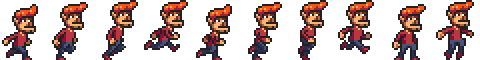
\includegraphics[width=6cm]{img/player_big.png}
\vskip 1.5ex\index{animation!platform game}

By alternating which pose we draw, we can show an animation that looks like a walking character.\index{fillRect method}\index{clearRect method}\index{clearing}

To animate a \index{picture}picture on a \index{canvas}canvas, the \lstinline`clearRect` method is useful. It resembles \lstinline`fillRect`, but instead of coloring the rectangle, it makes it \index{transparent}transparent, removing the previously drawn pixels.\index{setInterval function}\index{img (HTML tag)}

We know that each \emph{\index{sprite}sprite}, each subpicture, is 24 \index{pixel}pixels wide and 30 pixels high. The following code loads the image and then sets up an interval (repeated timer) to draw the next \index{frame}frame:

\begin{lstlisting}
<canvas></canvas>
<script>
  let cx = document.querySelector("canvas").getContext("2d");
  let img = document.createElement("img");
  img.src = "img/player.png";
  let spriteW = 24, spriteH = 30;
  img.addEventListener("load", () => {
    let cycle = 0;
    setInterval(() => {
      cx.clearRect(0, 0, spriteW, spriteH);
      cx.drawImage(img,
                   // source rectangle
                   cycle * spriteW, 0, spriteW, spriteH,
                   // destination rectangle
                   0,               0, spriteW, spriteH);
      cycle = (cycle + 1) % 8;
    }, 120);
  });
</script>
\end{lstlisting}
\noindent\index{remainder operator}\index{\% operator}\index{animation!platform game}

The \lstinline`cycle` binding tracks our position in the animation. For each \index{frame}frame, it is incremented and then clipped back to the 0 to 7 range by using the remainder operator. This binding is then used to compute the x-coordinate that the sprite for the current pose has in the picture.

\section{Transformation}\index{transformation}\index{mirroring}\index{flipping|see{mirroring}}

But what if we want our character to walk to the left instead of to the right? We could draw another set of sprites, of course. But we can also instruct the \index{canvas}canvas to draw the picture the other way round.\index{scale method}\index{scaling}

Calling the \lstinline`scale` method will cause anything drawn after it to be scaled. This method takes two parameters, one to set a horizontal scale and one to set a vertical scale.

\begin{lstlisting}
<canvas></canvas>
<script>
  let cx = document.querySelector("canvas").getContext("2d");
  cx.scale(3, .5);
  cx.beginPath();
  cx.arc(50, 50, 40, 0, 7);
  cx.lineWidth = 3;
  cx.stroke();
</script>
\end{lstlisting}
\noindent

Because of the call to \lstinline`scale`, the circle is drawn three times as wide and half as high.

\vskip 1.5ex
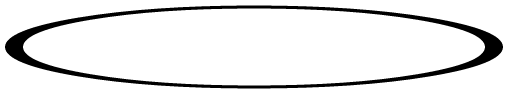
\includegraphics[width=6.6cm]{img/canvas_scale.png}
\vskip 1.5ex\index{mirroring}

Scaling will cause everything about the drawn image, including the \index{line width}line width, to be stretched out or squeezed together as specified. Scaling by a negative amount will flip the picture around. The flipping happens around point (0,0), which means it will also flip the direction of the coordinate system. When a horizontal scaling of -1 is applied, a shape drawn at x position 100 will end up at what used to be position -100.\index{drawImage method}

So to turn a picture around, we can't simply add \lstinline`cx.scale(-1, 1)` before the call to \lstinline`drawImage` because that would move our picture outside of the \index{canvas}canvas, where it won't be visible. You could adjust the \index{coordinates}coordinates given to \lstinline`drawImage` to compensate for this by drawing the image at x position -50 instead of 0. Another solution, which doesn't require the code that does the drawing to know about the scale change, is to adjust the \index{axis}axis around which the scaling happens.\index{rotate method}\index{translate method}\index{transformation}

There are several other methods besides \lstinline`scale` that influence the coordinate system for a \index{canvas}canvas. You can rotate subsequently drawn shapes with the \lstinline`rotate` method and move them with the \lstinline`translate` method. The interesting—and confusing—thing is that these transformations \emph{stack}, meaning that each one happens relative to the previous transformations.\index{rotate method}\index{translate method}

So if we translate by 10 horizontal pixels twice, everything will be drawn 20 pixels to the right. If we first move the center of the coordinate system to (50,50) and then rotate by 20 \index{degree}degrees (about 0.1π \index{radian}radians), that rotation will happen \emph{around} point (50,50).

\vskip 1.5ex
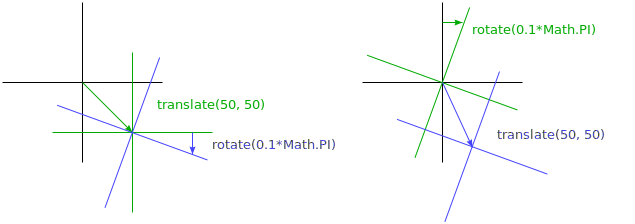
\includegraphics[width=9cm]{img/generated/transform.pdf}
\vskip 1.5ex\index{coordinates}

But if we \emph{first} rotate by 20 degrees and \emph{then} translate by (50,50), the translation will happen in the rotated coordinate system and thus produce a different orientation. The order in which transformations are applied matters.\index{axis}\index{mirroring}

To flip a picture around the vertical line at a given x position, we can do the following:

\begin{lstlisting}
function flipHorizontally(context, around) {
  context.translate(around, 0);
  context.scale(-1, 1);
  context.translate(-around, 0);
}
\end{lstlisting}
\noindent\index{flipHorizontally method}

We move the y-\index{axis}axis to where we want our \index{mirror}mirror to be, apply the mirroring, and finally move the y-axis back to its proper place in the mirrored universe. The following picture explains why this works:

\vskip 1.5ex
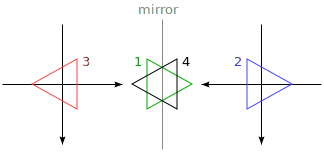
\includegraphics[width=8cm]{img/generated/mirror.pdf}
\vskip 1.5ex\index{translate method}\index{scale method}\index{transformation}\index{canvas}

This shows the coordinate systems before and after mirroring across the central line. The triangles are numbered to illustrate each step. If we draw a triangle at a positive x position, it would, by default, be in the place where triangle 1 is. A call to \lstinline`flipHorizontally` first does a translation to the right, which gets us to triangle 2. It then scales, flipping the triangle over to position 3. This is not where it should be, if it were mirrored in the given line. The second \lstinline`translate` call fixes this—it ``cancels'' the initial translation and makes triangle 4 appear exactly where it should.

We can now draw a mirrored character at position (100,0) by flipping the world around the character's vertical center.

\begin{lstlisting}
<canvas></canvas>
<script>
  let cx = document.querySelector("canvas").getContext("2d");
  let img = document.createElement("img");
  img.src = "img/player.png";
  let spriteW = 24, spriteH = 30;
  img.addEventListener("load", () => {
    flipHorizontally(cx, 100 + spriteW / 2);
    cx.drawImage(img, 0, 0, spriteW, spriteH,
                 100, 0, spriteW, spriteH);
  });
</script>
\end{lstlisting}
\noindent

\section{Storing and clearing transformations}\index{side effect}\index{canvas}\index{transformation}

Transformations stick around. Everything else we draw after \index{drawing}drawing that mirrored character would also be mirrored. That might be inconvenient.

It is possible to save the current transformation, do some drawing and transforming, and then restore the old transformation. This is usually the proper thing to do for a function that needs to temporarily transform the coordinate system. First, we save whatever transformation the code that called the function was using. Then the function does its thing, adding more transformations on top of the current transformation. Finally, we revert to the transformation we started with.\index{save method}\index{restore method}\index{state!of canvas}

The \lstinline`save` and \lstinline`restore` methods on the 2D \index{canvas}canvas context do this \index{transformation}transformation management. They conceptually keep a stack of transformation states. When you call \lstinline`save`, the current state is pushed onto the stack, and when you call \lstinline`restore`, the state on top of the stack is taken off and used as the context's current transformation. You can also call \lstinline`resetTransform` to fully reset the transformation.\index{branching recursion}\index{fractal example}\index{recursion}

The \lstinline`branch` function in the following example illustrates what you can do with a function that changes the transformation and then calls a function (in this case itself), which continues drawing with the given transformation.

This function draws a treelike shape by drawing a line, moving the center of the coordinate system to the end of the line, and calling itself twice—first rotated to the left and then rotated to the right. Every call reduces the length of the branch drawn, and the recursion stops when the length drops below 8.

\begin{lstlisting}
<canvas width="600" height="300"></canvas>
<script>
  let cx = document.querySelector("canvas").getContext("2d");
  function branch(length, angle, scale) {
    cx.fillRect(0, 0, 1, length);
    if (length < 8) return;
    cx.save();
    cx.translate(0, length);
    cx.rotate(-angle);
    branch(length * scale, angle, scale);
    cx.rotate(2 * angle);
    branch(length * scale, angle, scale);
    cx.restore();
  }
  cx.translate(300, 0);
  branch(60, 0.5, 0.8);
</script>
\end{lstlisting}
\noindent

The result is a simple fractal.

\vskip 1.5ex
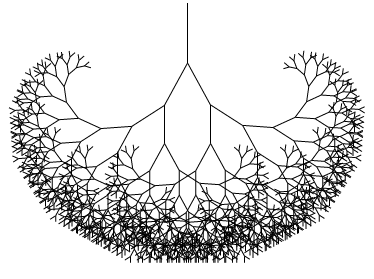
\includegraphics[width=5cm]{img/canvas_tree.png}
\vskip 1.5ex\index{save method}\index{restore method}\index{canvas}\index{rotate method}

If the calls to \lstinline`save` and \lstinline`restore` were not there, the second recursive call to \lstinline`branch` would end up with the position and rotation created by the first call. It wouldn't be connected to the current branch but rather to the innermost, rightmost branch drawn by the first call. The resulting shape might also be interesting, but it is definitely not a tree.

\label{canvas.canvasdisplay}\section{Back to the game}\index{drawImage method}

We now know enough about \index{canvas}canvas drawing to start working on a \index{canvas}canvas-based \index{display}display system for the \index{game}game from the \hyperref[game]{previous chapter}. The new display will no longer be showing just colored boxes. Instead, we'll use \lstinline`drawImage` to draw pictures that represent the game's elements.\index{CanvasDisplay class}\index{DOMDisplay class}\index{interface!object}

We define another display object type called \lstinline`CanvasDisplay`, supporting the same interface as \lstinline`DOMDisplay` from \hyperref[game.domdisplay]{Chapter 16}, namely, the methods \lstinline`syncState` and \lstinline`clear`.\index{state!in objects}

This object keeps a little more information than \lstinline`DOMDisplay`. Rather than using the scroll position of its DOM element, it tracks its own \index{viewport}viewport, which tells us what part of the level we are currently looking at. Finally, it keeps a \lstinline`flipPlayer` property so that even when the player is standing still, it keeps facing the direction it last moved in.

\begin{lstlisting}
class CanvasDisplay {
  constructor(parent, level) {
    this.canvas = document.createElement("canvas");
    this.canvas.width = Math.min(600, level.width * scale);
    this.canvas.height = Math.min(450, level.height * scale);
    parent.appendChild(this.canvas);
    this.cx = this.canvas.getContext("2d");

    this.flipPlayer = false;

    this.viewport = {
      left: 0,
      top: 0,
      width: this.canvas.width / scale,
      height: this.canvas.height / scale
    };
  }

  clear() {
    this.canvas.remove();
  }
}
\end{lstlisting}
\noindent

The \lstinline`syncState` method first computes a new viewport and then draws the game scene at the appropriate position.

\begin{lstlisting}
CanvasDisplay.prototype.syncState = function(state) {
  this.updateViewport(state);
  this.clearDisplay(state.status);
  this.drawBackground(state.level);
  this.drawActors(state.actors);
};
\end{lstlisting}
\noindent\index{scrolling}\index{clearing}

Contrary to \lstinline`DOMDisplay`, this display style \emph{does} have to redraw the background on every update. Because shapes on a canvas are just \index{pixel}pixels, after we draw them there is no good way to move them (or remove them). The only way to update the canvas display is to clear it and redraw the scene. We may also have scrolled, which requires the background to be in a different position.\index{CanvasDisplay class}

The \lstinline`updateViewport` method is similar to \lstinline`DOMDisplay`'s \lstinline`scrollPlayerIntoView` method. It checks whether the player is too close to the edge of the screen and moves the \index{viewport}viewport when this is the case.

\begin{lstlisting}
CanvasDisplay.prototype.updateViewport = function(state) {
  let view = this.viewport, margin = view.width / 3;
  let player = state.player;
  let center = player.pos.plus(player.size.times(0.5));

  if (center.x < view.left + margin) {
    view.left = Math.max(center.x - margin, 0);
  } else if (center.x > view.left + view.width - margin) {
    view.left = Math.min(center.x + margin - view.width,
                         state.level.width - view.width);
  }
  if (center.y < view.top + margin) {
    view.top = Math.max(center.y - margin, 0);
  } else if (center.y > view.top + view.height - margin) {
    view.top = Math.min(center.y + margin - view.height,
                        state.level.height - view.height);
  }
};
\end{lstlisting}
\noindent\index{boundary}\index{Math.max function}\index{Math.min function}\index{clipping}

The calls to \lstinline`Math.max` and \lstinline`Math.min` ensure that the viewport does not end up showing space outside of the level. \lstinline`Math.max(x, 0)` makes sure the resulting number is not less than zero. \lstinline`Math.min` similarly guarantees that a value stays below a given bound.

When \index{clearing}clearing the display, we'll use a slightly different \index{color}color depending on whether the game is won (brighter) or lost (darker).

\begin{lstlisting}
CanvasDisplay.prototype.clearDisplay = function(status) {
  if (status == "won") {
    this.cx.fillStyle = "rgb(68, 191, 255)";
  } else if (status == "lost") {
    this.cx.fillStyle = "rgb(44, 136, 214)";
  } else {
    this.cx.fillStyle = "rgb(52, 166, 251)";
  }
  this.cx.fillRect(0, 0,
                   this.canvas.width, this.canvas.height);
};
\end{lstlisting}
\noindent\index{Math.floor function}\index{Math.ceil function}\index{rounding}

To draw the background, we run through the tiles that are visible in the current viewport, using the same trick used in the \lstinline`touches` method from the \hyperref[game.touches]{previous chapter}.

\begin{lstlisting}
let otherSprites = document.createElement("img");
otherSprites.src = "img/sprites.png";

CanvasDisplay.prototype.drawBackground = function(level) {
  let {left, top, width, height} = this.viewport;
  let xStart = Math.floor(left);
  let xEnd = Math.ceil(left + width);
  let yStart = Math.floor(top);
  let yEnd = Math.ceil(top + height);

  for (let y = yStart; y < yEnd; y++) {
    for (let x = xStart; x < xEnd; x++) {
      let tile = level.rows[y][x];
      if (tile == "empty") continue;
      let screenX = (x - left) * scale;
      let screenY = (y - top) * scale;
      let tileX = tile == "lava" ? scale : 0;
      this.cx.drawImage(otherSprites,
                        tileX,         0, scale, scale,
                        screenX, screenY, scale, scale);
    }
  }
};
\end{lstlisting}
\noindent\index{drawImage method}\index{sprite}\index{tile}

Tiles that are not empty are drawn with \lstinline`drawImage`. The \lstinline`otherSprites` image contains the pictures used for elements other than the player. It contains, from left to right, the wall tile, the lava tile, and the sprite for a coin.

\vskip 1.5ex
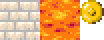
\includegraphics[width=1.4cm]{img/sprites_big.png}
\vskip 1.5ex\index{scaling}

Background tiles are 20 by 20 pixels since we will use the same scale that we used in \lstinline`DOMDisplay`. Thus, the offset for lava tiles is 20 (the value of the \lstinline`scale` binding), and the offset for walls is 0.\index{drawing}\index{load event}\index{drawImage method}

We don't bother waiting for the sprite image to load. Calling \lstinline`drawImage` with an image that hasn't been loaded yet will simply do nothing. Thus, we might fail to draw the game properly for the first few \index{frame}frames, while the image is still loading, but that is not a serious problem. Since we keep updating the screen, the correct scene will appear as soon as the loading finishes.\index{player}\index{animation!platform game}\index{drawing}

The \index{walking}walking character shown earlier will be used to represent the player. The code that draws it needs to pick the right \index{sprite}sprite and direction based on the player's current motion. The first eight sprites contain a walking animation. When the player is moving along a floor, we cycle through them based on the current time. We want to switch frames every 60 milliseconds, so the \index{time}time is divided by 60 first. When the player is standing still, we draw the ninth sprite. During jumps, which are recognized by the fact that the vertical speed is not zero, we use the tenth, rightmost sprite.\index{flipHorizontally function}\index{CanvasDisplay class}

Because the \index{sprite}sprites are slightly wider than the player object—24 instead of 16 pixels to allow some space for feet and arms—the method has to adjust the x-coordinate and width by a given amount (\lstinline`playerXOverlap`).

\begin{lstlisting}
let playerSprites = document.createElement("img");
playerSprites.src = "img/player.png";
const playerXOverlap = 4;

CanvasDisplay.prototype.drawPlayer = function(player, x, y,
                                              width, height){
  width += playerXOverlap * 2;
  x -= playerXOverlap;
  if (player.speed.x != 0) {
    this.flipPlayer = player.speed.x < 0;
  }

  let tile = 8;
  if (player.speed.y != 0) {
    tile = 9;
  } else if (player.speed.x != 0) {
    tile = Math.floor(Date.now() / 60) % 8;
  }

  this.cx.save();
  if (this.flipPlayer) {
    flipHorizontally(this.cx, x + width / 2);
  }
  let tileX = tile * width;
  this.cx.drawImage(playerSprites, tileX, 0, width, height,
                                   x,     y, width, height);
  this.cx.restore();
};
\end{lstlisting}
\noindent

The \lstinline`drawPlayer` method is called by \lstinline`drawActors`, which is responsible for drawing all the actors in the game.

\begin{lstlisting}
CanvasDisplay.prototype.drawActors = function(actors) {
  for (let actor of actors) {
    let width = actor.size.x * scale;
    let height = actor.size.y * scale;
    let x = (actor.pos.x - this.viewport.left) * scale;
    let y = (actor.pos.y - this.viewport.top) * scale;
    if (actor.type == "player") {
      this.drawPlayer(actor, x, y, width, height);
    } else {
      let tileX = (actor.type == "coin" ? 2 : 1) * scale;
      this.cx.drawImage(otherSprites,
                        tileX, 0, width, height,
                        x,     y, width, height);
    }
  }
};
\end{lstlisting}
\noindent

When \index{drawing}drawing something that is not the \index{player}player, we look at its type to find the offset of the correct sprite. The \index{lava}lava tile is found at offset 20, and the \index{coin}coin sprite is found at 40 (two times \lstinline`scale`).\index{viewport}

We have to subtract the viewport's position when computing the actor's position since (0,0) on our \index{canvas}canvas corresponds to the top left of the viewport, not the top left of the level. We could also have used \lstinline`translate` for this. Either way works.\index{game!screenshot}\index{game!with canvas}

That concludes the new \index{display}display system. The resulting game looks something like this:

\vskip 1.5ex
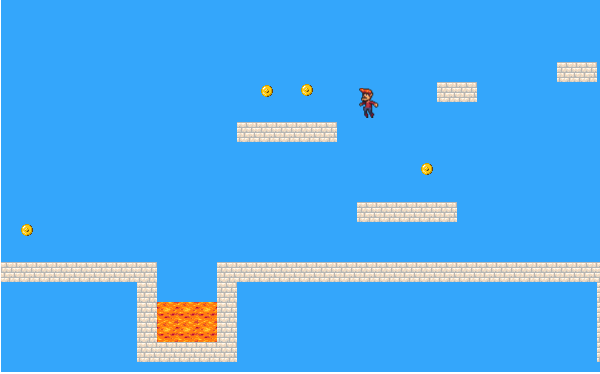
\includegraphics[width=8cm]{img/canvas_game.png}
\vskip 1.5ex

\label{canvas.graphics_tradeoffs}\section{Choosing a graphics interface}

So when you need to generate graphics in the browser, you can choose between plain HTML, \index{SVG}SVG, and \index{canvas}canvas. There is no single \emph{best} approach that works in all situations. Each option has strengths and weaknesses.\index{text wrapping}

Plain HTML has the advantage of being simple. It also integrates well with \index{text}text. Both SVG and canvas allow you to draw text, but they won't help you position that text or wrap it when it takes up more than one line. In an HTML-based picture, it is much easier to include blocks of text.\index{zooming}\index{SVG}

SVG can be used to produce \index{crisp}crisp \index{graphics}graphics that look good at any zoom level. Unlike HTML, it is designed for drawing and is thus more suitable for that purpose.\index{DOM!graphics}\index{SVG}\index{event handling}\index{data structure!tree}

Both SVG and HTML build up a data structure (the DOM) that represents your picture. This makes it possible to modify elements after they are drawn. If you need to repeatedly change a small part of a big \index{picture}picture in response to what the user is doing or as part of an \index{animation}animation, doing it in a canvas can be needlessly expensive. The DOM also allows us to register mouse event handlers on every element in the picture (even on shapes drawn with SVG). You can't do that with canvas.\index{performance}\index{optimization}

But \index{canvas}canvas's \index{pixel}pixel-oriented approach can be an advantage when drawing a huge number of tiny elements. The fact that it does not build up a data structure but only repeatedly draws onto the same pixel surface gives canvas a lower cost per shape.\index{ray tracer}

There are also effects, such as rendering a scene one pixel at a time (for example, using a ray tracer) or postprocessing an image with JavaScript (blurring or distorting it), that can be realistically handled only by a \index{pixel}pixel-based approach.

In some cases, you may want to combine several of these techniques. For example, you might draw a \index{graph}graph with \index{SVG}SVG or \index{canvas}canvas but show \index{text}textual information by positioning an HTML element on top of the picture.\index{display}

For nondemanding applications, it really doesn't matter much which interface you choose. The display we built for our game in this chapter could have been implemented using any of these three \index{graphics}graphics technologies since it does not need to draw text, handle mouse interaction, or work with an extraordinarily large number of elements.

\section{Summary}

In this chapter we discussed techniques for drawing graphics in the browser, focusing on the \lstinline`<canvas>` element.

A canvas node represents an area in a document that our program may draw on. This drawing is done through a drawing context object, created with the \lstinline`getContext` method.

The 2D drawing interface allows us to fill and stroke various shapes. The context's \lstinline`fillStyle` property determines how shapes are filled. The \lstinline`strokeStyle` and \lstinline`lineWidth` properties control the way lines are drawn.

Rectangles and pieces of text can be drawn with a single method call. The \lstinline`fillRect` and \lstinline`strokeRect` methods draw rectangles, and the \lstinline`fillText` and \lstinline`strokeText` methods draw text. To create custom shapes, we must first build up a path.\index{stroking}\index{filling}

Calling \lstinline`beginPath` starts a new path. A number of other methods add lines and curves to the current path. For example, \lstinline`lineTo` can add a straight line. When a path is finished, it can be filled with the \lstinline`fill` method or stroked with the \lstinline`stroke` method.

Moving pixels from an image or another canvas onto our canvas is done with the \lstinline`drawImage` method. By default, this method draws the whole source image, but by giving it more parameters, you can copy a specific area of the image. We used this for our game by copying individual poses of the game character out of an image that contained many such poses.

Transformations allow you to draw a shape in multiple orientations. A 2D drawing context has a current transformation that can be changed with the \lstinline`translate`, \lstinline`scale`, and \lstinline`rotate` methods. These will affect all subsequent drawing operations. A transformation state can be saved with the \lstinline`save` method and restored with the \lstinline`restore` method.

When showing an animation on a canvas, the \lstinline`clearRect` method can be used to clear part of the canvas before redrawing it.

\section{Exercises}

\subsection{Shapes}\index{shapes (exercise)}

Write a program that draws the following \index{shape}shapes on a \index{canvas}canvas:\index{rotation}

\begin{enumerate}
\item 

A \index{trapezoid}trapezoid (a \index{rectangle}rectangle that is wider on one side)
\item 

A red \index{diamond}diamond (a rectangle rotated 45 degrees or ¼π radians)
\item 

A zigzagging \index{line}line
\item 

A \index{spiral}spiral made up of 100 straight line segments
\item 

A yellow \index{star}star
\end{enumerate}

\vskip 1.5ex
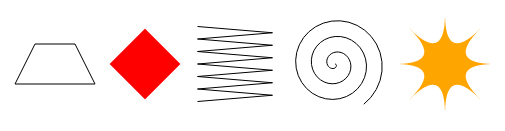
\includegraphics[width=8cm]{img/exercise_shapes.png}
\vskip 1.5ex

When drawing the last two, you may want to refer to the explanation of \lstinline`Math.cos` and \lstinline`Math.sin` in \hyperref[dom.sin_cos]{Chapter 14}, which describes how to get coordinates on a circle using these functions.\index{readability}\index{hard-coding}

I recommend creating a function for each shape. Pass the position, and optionally other properties such as the size or the number of points, as parameters. The alternative, which is to hard-code numbers all over your code, tends to make the code needlessly hard to read and modify.

\label{canvas.exercise_pie_chart}\subsection{The pie chart}\index{label}\index{text}\index{pie chart example}

\hyperref[canvas.pie_chart]{Earlier} in the chapter, we saw an example program that drew a pie chart. Modify this program so that the name of each category is shown next to the slice that represents it. Try to find a pleasing-looking way to automatically position this text that would work for other data sets as well. You may assume that categories are big enough to leave ample room for their labels.

You might need \lstinline`Math.sin` and \lstinline`Math.cos` again, which are described in \hyperref[dom.sin_cos]{Chapter 14}.

\subsection{A bouncing ball}\index{animation!bouncing ball}\index{requestAnimationFrame function}\index{bouncing}

Use the \lstinline`requestAnimationFrame` technique that we saw in \hyperref[dom.animationFrame]{Chapter 14} and \hyperref[game.runAnimation]{Chapter 16} to draw a \index{box}box with a bouncing \index{ball}ball in it. The ball moves at a constant \index{speed}speed and bounces off the box's sides when it hits them.

\subsection{Precomputed mirroring}\index{optimization}\index{bitmap graphics}\index{mirror}

One unfortunate thing about \index{transformation}transformations is that they slow down the drawing of bitmaps. The position and size of each \index{pixel}pixel has to be transformed, and though it is possible that \index{browser}browsers will get cleverer about transformation in the \index{future}future, they currently cause a measurable increase in the time it takes to draw a bitmap.

In a game like ours, where we are drawing only a single transformed sprite, this is a nonissue. But imagine that we need to draw hundreds of characters or thousands of rotating particles from an explosion.

Think of a way to allow us to draw an inverted character without loading additional image files and without having to make transformed \lstinline`drawImage` calls every frame.
